\documentclass[10pt]{beamer}

\usetheme[progressbar=frametitle, numbering=fraction,]{metropolis}

\usepackage{booktabs}
\usepackage{pgfplots}
\usepgfplotslibrary{dateplot}
\usepackage{texshade}      
\usepackage{amsmath}
\usepackage{amssymb}
\usepackage{xspace}
\usepackage{xcolor}
\usepackage{appendixnumberbeamer}
\usepackage{multirow}
\usepackage{verbatim}

\usepackage{tikz}
\usetikzlibrary{shapes.geometric, arrows}
\tikzstyle{startstop} = [rectangle, rounded corners, minimum width=3cm, minimum height=1cm,text centered, draw=black, fill=red!30]
\tikzstyle{io} = [trapezium, trapezium left angle=70, trapezium right angle=110, minimum width=3cm, minimum height=1cm, text centered, draw=black, fill=blue!30]
\tikzstyle{process} = [rectangle, minimum width=3cm, minimum height=1cm, text centered, draw=black, fill=orange!30]
\tikzstyle{decision} = [diamond, minimum width=3cm, minimum height=1cm, text centered, draw=black, fill=green!30]

\tikzstyle{arrow} = [thick,->,>=stealth]


\newcommand{\themename}{\textbf{\textsc{metropolis}}\xspace}

\setbeamercovered{invisible}
\setbeamertemplate{caption}{\raggedright\insertcaption\par}

\title{Dissection Of Sheep Brain}
%\subtitle{What we see, is not what it is}
\date{\today}
\author{Saket Choudhary}
\institute{BISC 104\\Session 5}
%\titlegraphic{\hfill
\includegraphics[height=1.5cm]{logo}}

\begin{document}

\maketitle

\begin{frame}{Todays' Experiment}
\begin{itemize}[<+-| alert@+>]
\item Dissecting a sheep's brain
\item Completely exploratory!
\item Try finding all parts/regions mentioned in your handout
\end{itemize}

\end{frame}

\begin{frame}[fragile]{Brain Regions}
\begin{figure}
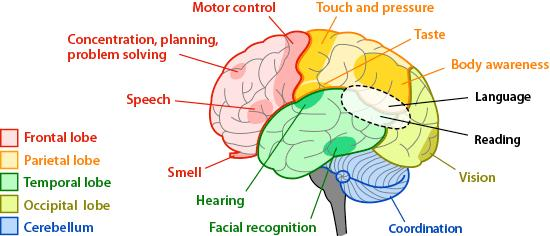
\includegraphics[width=\linewidth]{brain.jpg}
\end{figure}
$https://www.youtube.com/watch?v=vE3Yf_xy_mE$
\end{frame}

\begin{frame}[fragile]{Brain Regions}
%\begin{minipage}{0.5\linewidth}
\begin{figure}
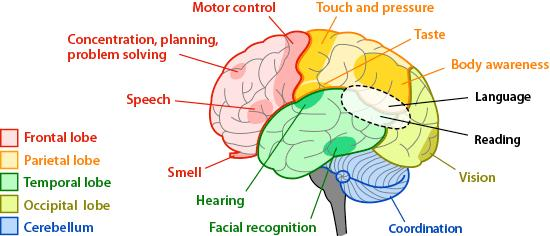
\includegraphics[width=0.5\linewidth]{brain.jpg}
\end{figure}
%\end{minipage}
%\begin{minipage}{0.5\linewidth}
\begin{itemize}[<+-| alert@+>]
\item Frontal: Movement, speech, coordination, judgement
\item Parietal: Touch, pressure
\item Temporal: Memory, hearing
\item Occipital: vision
\end{itemize}
%\end{minipage}
\end{frame}

\begin{frame}[fragile]{Some other structures}
\begin{figure}
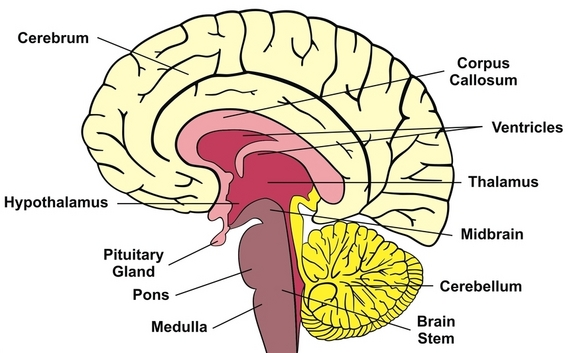
\includegraphics[width=0.5\linewidth]{deeper.jpg}
\end{figure}
\begin{itemize}[<+-| alert@+>]
\item Hypothalamus: Hunger, thirst, sexual response
\item Pituitary gland: "Master gland"
\item Cerebrum: Largest part of brain
\item Cerebellum: "little brain": attention, language
\item Pons: forebrain to cerebellum signalling
\end{itemize}
\end{frame}




\begin{frame}[fragile]{Office Hours}
\Large \begin{center}Tuesday: 9-10AM\\
Thursday: 9-10AM\\
ZSH 372\\
\vspace*{2cm}
Saket Choudhary\\ 
skchoudh@usc.edu\\
\end{center}


\end{frame}

\end{document}
